\section{Network-On-Chip (NoC)}

\sh{Evolution of Buses}
A network-on-chip is a communication system used in modern \ac{SoC} architectures to efficiently connect various components (e.g., processors, memory, and specialized units). Instead of using classic buses or point-to-point connections, \ac{NoC} relies on a network-like communication principle inspired by computer networks or high-performance computers.\cite{serpanos_architecture_2011}

The Fig.~\ref{fig:Evolution_of_Interconnection} shows the development of bus technologies over the past few years.
\begin{figure}[htbp]
    \centering
    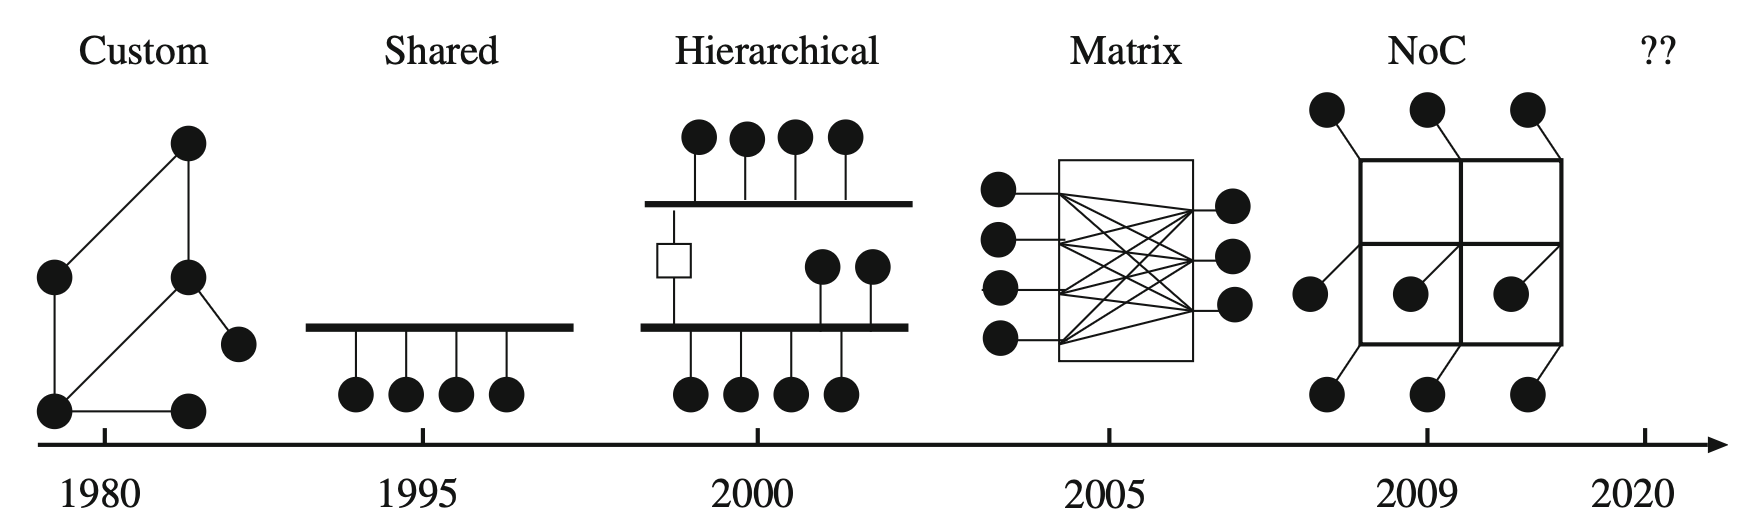
\includegraphics[width=0.95\textwidth]{img/Evolution of On-Chip communication interconnect.png}
    \caption{Evolution of Interconnections}~\cite{abderazek_multicore_2013}\label{fig:Evolution_of_Interconnection}
\end{figure}

Before 1980, custom solutions were typically used for on-chip communication. Starting around 1995, so-called shared-bus architectures such as ARM’s AMBA bus \cite{arm_amba_nodate} and IBM’s CoreConnect\cite{international_business_machines_corporation_coreconnect_1999} were introduced. These approaches enabled a more modular design with standardized interfaces and supported the reuse of IP components (IP reuse).
However, as bandwidth demands increased, shared-bus systems became a bottleneck. To address this issue, hierarchical bus architectures were introduced. These utilize multiple buses or bus segments to reduce the load on the main bus. Local communication between modules on the same bus segment is possible without burdening the entire bus. Nevertheless, such architectures are only limitedly scalable, inflexible, and lead to increased design complexity. The more cores are connected, the harder it becomes to meet timing constraints (time closure\footnote{Time Closure: Successfully ensuring all timing constraints are satisfied in the design so that the chip can operate reliably at its target clock frequency.}) and ensure \ac{QoS}.
Another alternative was the bus matrix — a full crossbar system that allows parallel connections between components. However, as system size grows, the complexity of wiring also increases and can eventually improve the effort required for the logic itself. Moreover, such systems do not clearly separate transport, transaction, and physical layers. Therefore, when a system upgrade is needed, it often affects the entire interface design and all connected blocks.
Against this background, some researchers in the early 2000s proposed implementing communication between different processing units on a chip via a predefined platform—an integrated switching network known as Network-on-Chip. NoCs fulfill key requirements of modern \ac{SoC}s: Reusability, scalable bandwidth, and energy efficiency. NoCs have replaced wired connections and instead utilize intelligent network infrastructures. They draw on models, techniques, and tools from network communication, thereby replacing fixed wiring with packet-based communication.\cite{unnikrishnan_network_2021}


\sh{NoC Components}
A \ac{NoC} consists of the following three essential components:\cite{yu_flexible_2010}\cite{unnikrishnan_network_2021}
\begin{enumerate}
    \item \textbf{Links}, which physically connect the nodes and enable communication between them. A link connects exactly two routers (see item 2). A link can contain one or more logical channels; a channel in turn consists of a set of wires (cables). The implementation of a link also includes the definition of the synchronization protocol between the source and the destination node.
    \item \textbf{Routers}, which are responsible for implementing the communication protocol. A router has multiple input and output ports as well as a switching matrix that establishes the connection between these ports. Additionally, each router has a local port connected to the respective IP core. A logic block inside the router controls the flow control (see below for further description) policies and defines the overall strategy for data forwarding.
    \item \textbf{\ac{NA}} or \textbf{\ac{NI}} serve as the logical interface between the IP cores and the network. They are necessary because the internal communication mechanisms of an IP core (e.g. bus protocols like AXI) are typically not directly compatible with the packet-based mechanisms of a \ac{NoC}.
\end{enumerate}


\sh{Topology}
\ac{NoC} can be characterized by the structure of their router connections. This structure is also referred to as the \textit{topology} and is typically represented as a graph $G(N, C)$, where $N$ denotes the set of routers (nodes) and $C$ the set of channels (edges). A fundamental distinction is made between \textit{direct} and \textit{indirect topology}.
In the case of \textit{direct topology}, each router is assigned exactly one processor. This pair is considered a node in the network. Each node is connected to a fixed number of neighbors, and messages are transported over one or more intermediate nodes (routers). Commonly used structures include n-dimensional grids, mesh topologies, or torus topologies (also called k-ary n-cubes).
In \textit{indirect topology}, not all routers are directly connected to a processing unit, as is the case in the direct model. Some routers serve solely to route messages through the network, while others are responsible for control and management functions. These so-called logic routers act as sources or targets of messages.\cite{unnikrishnan_network_2021}


\sh{Routing}
In NoC architectures, routing is a central component because it determines how data packets are transmitted between individual nodes. Fundamentally, routing algorithms can be divided into two main categories: deterministic and adaptive routing. In \textit{deterministic routing}, the path a packet takes from the source to the destination is predefined and remains unchanged regardless of the current network load or other conditions. Well-known deterministic methods include XY-routing and \ac{DOR}.\cite{ma_summary_2024} In contrast, \textit{adaptive routing} allows dynamic path adjustments based on the current state of the network. This enables, for example, the avoidance of congestion or faulty connections. Adaptive algorithms include \ac{DyAD}\cite{hu_dyad_2004} as well as Odd-Even routing.

Complementing these are \textit{congestion-aware routing algorithms} that specifically consider the current network load to achieve an even distribution of data traffic.\cite{fang_parrouting_2020} A special subcategory are so-called \textit{ant colony-based algorithms}, which use concepts from swarm intelligence. Here, paths are learned and continuously optimized using virtual pheromone trails, enabling flexible and adaptive route finding.\cite{luneque_routing_2013}


\sh{Flow Control}
Another essential aspect in NoC systems is the so-called flow control, which defines how available resources such as bandwidth or buffer memory are assigned to individual data packets. The goal is to ensure efficient resource usage and thereby optimize the overall network throughput. Fundamentally, one distinguishes between bufferless and buffered flow control. In \textit{bufferless flow control}, there are no or only very limited intermediate storage; data packets that cannot be forwarded immediately are either discarded or rerouted via alternative paths. A typical example is circuit switching, where a fixed path through the network is reserved prior to data transmission. In contrast, buffered flow control temporarily stores data packets when the desired output channel is occupied or forwarding is otherwise delayed. This method increases the flexibility of data transmission and reduces the likelihood of packet loss or rerouting, but entails higher hardware complexity and energy consumption due to the additional buffer resources that must be provided and managed.

Within \textit{buffered flow control}, two central approaches can be distinguished: In packet-buffer flow control, the entire packet is stored in a buffer until it can be forwarded completely. This method is simple to implement but can be inefficient, especially for large packets and limited buffer memory. A finer control is provided by flit-buffer flow control, where packets are divided into smaller units called flits (flow control digits) and buffered individually. This allows more efficient use of available memory and better coordination of data flow, potentially leading to higher network performance.

Additionally, different buffering strategies exist within these approaches, including \textit{input buffering}, \textit{output buffering}, and \textit{virtual channel buffering}. Input buffering stores incoming data streams at each input channel, while output buffering places buffers at the router’s output channels. Virtual channel buffering allows multiple logical channels to share one physical channel, thereby reducing blocking and improving the utilization of available bandwidth. However, this technique requires more complex control logic and increases hardware overhead.\cite{dally_principles_2004}

\begin{figure}[htbp]
    \centering
    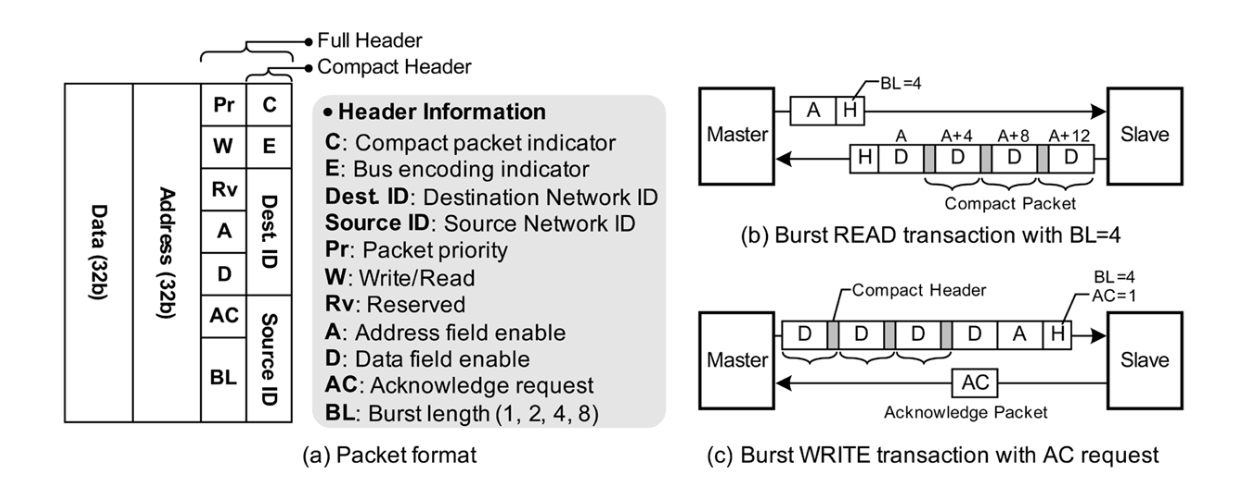
\includegraphics[width=0.95\textwidth]{img/NoC Protocol.png}
    \caption{NoC-Protocol~\cite{lee_low-power_2006}}\label{fig:NOC_Protocol}
\end{figure}


\sh{Protocol}
The network protocol for the Network-on-Chip (NoC) presented in \cite{lee_low-power_2006} was developed with the goal of enabling both high data transfer efficiency and low power consumption. The basis is a flexibly structured packet format with a modular header, which can be divided into a full or compact header as needed. The header includes, among other things, information about packet priority (Pr), transfer mode (Read/Write), burst length (BL), source and destination addresses (Source/Dest ID), as well as optional fields such as address or data activation (A, D) and an acknowledge request (AC).

Burst communication typically occurs with a burst length of 1, 2, 4, or 8 transfers. In a \emph{Burst READ} (see Fig.~\ref{fig:NOC_Protocol}), the master first sends a packet with the address and full header to the slave. The slave then responds with multiple compact packets, each containing one data word. The re-transmission of address information is omitted because it can be derived from the initial address and the burst length. In contrast, during a \emph{Burst WRITE}, the master sends multiple data packets together with a compact header and the destination address to the slave. Optionally, an acknowledge request can be set, so that the slave sends back a confirmation packet (ACK) after successful reception.

The structure of the protocol allows minimizing overhead and reducing energy consumption by using compact headers and selective field activation. Particularly noteworthy is the combination of efficient data transfer, scalability, and hardware friendliness, which makes this protocol well suited for use in high-performance and energy-optimized system-on-chip architectures.

However, it should be noted that the protocol presented here is only one example from the multitude of existing NoC communication protocols. Depending on the use case and system requirements, different protocols exist that are optimized, for example, for different flow control mechanisms, routing strategies, or real-time requirements. NoC protocols vary significantly in header structure, burst support, energy efficiency, and error handling to meet specific design goals. Therefore, the choice of a NoC protocol is always adapted to the particular requirements of the target system.


\sh{Advantages and Disadvantages}
A Network-on-Chip (NoC) offers several advantages over traditional bus-based communication structures: It enables scalable and parallel data transfer between many processor cores or components, significantly improving performance and efficiency in complex systems. Moreover, the structured interconnection enhances fault tolerance and bandwidth while reducing latency.

However, NoCs also bring disadvantages, such as increased design and implementation effort, as well as additional chip area and power consumption. In particular, the complexity of routing and control can complicate development and validation. Overall, however, in modern multicore systems the advantages of NoCs usually outweigh the disadvantages, as they provide a flexible and high-performance communication infrastructure.\cite{dally_principles_2004}
